\subsection{یخش پ}
ضرایب حلقه هدایت در جدول پایین آورده شده است.


\begin{table}[H]
	\caption{ضرایب حلقه هدایت و فاصله ازدست‌دهی همراه با مشتق‌گیر }
	\centering
	\begin{tabular}{cc}
		\hline
		Value &  Parameter \\
		\hline
		\lr{95.2874} & \lr{$k_{\epsilon}$}\\
		\lr{10} & \lr{$d_{\epsilon}$}\\
		\lr{50.5153}  & \lr{$k_{\sigma}$}\ \\ 
		\lr{10}  & \lr{$d_{\sigma}$}\ \\ 
		\lr{0.6711}& \lr{Miss Distance(m)}  \\
		\hline
	\end{tabular}
\end{table}

نتایج شبیه‌سازی در پایین آورده شده است.

\begin{figure}[H]
	\centering
	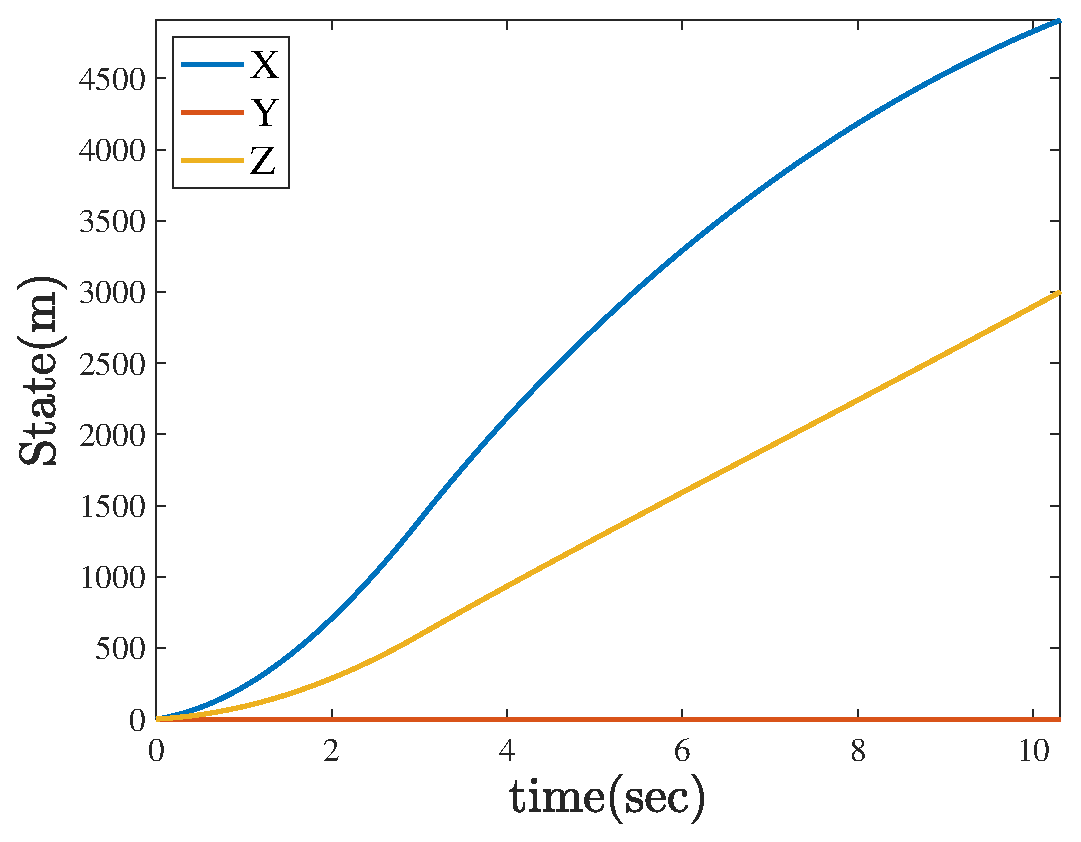
\includegraphics[width=.75\linewidth]{../Figure/d/missle_state}
	\caption{موقعیت موشک در هدایت خط دید پایه همراه با مشتق‌گیر}
\end{figure}

\begin{figure}[H]
	\centering
	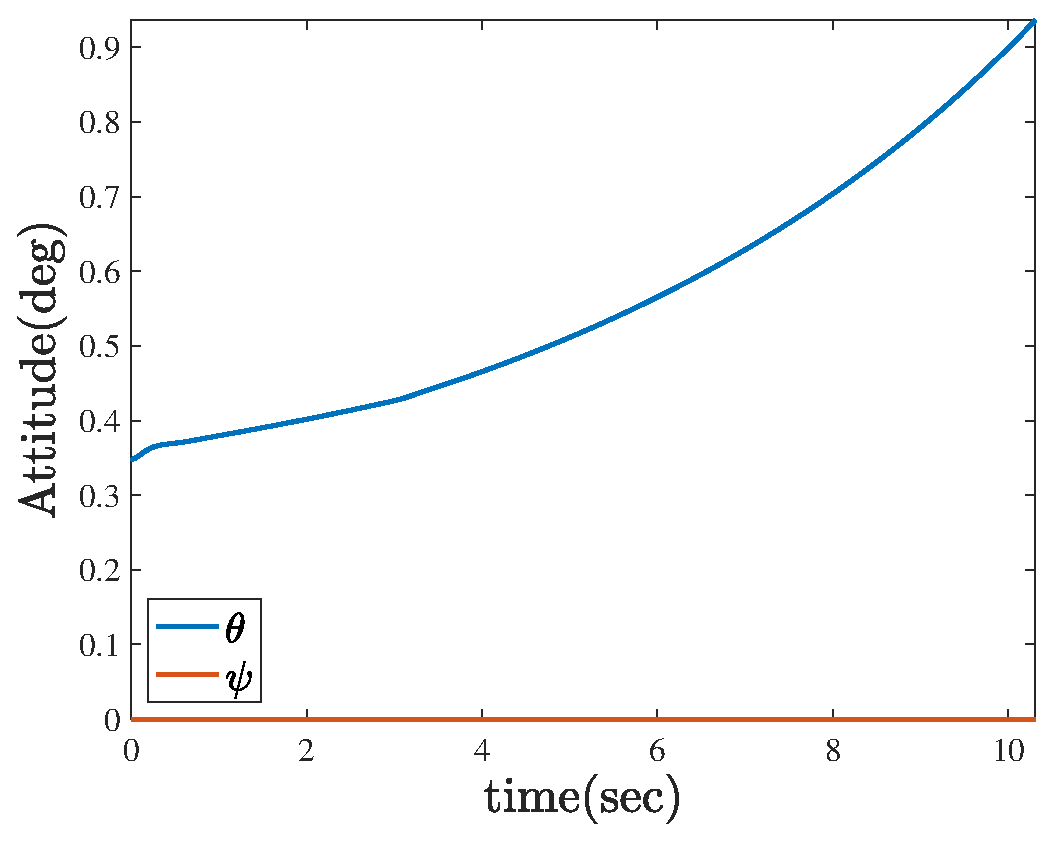
\includegraphics[width=.75\linewidth]{../Figure/d/missle_attitude}
	\caption{وضعیت موشک  در هدایت خط دید پایه همراه با مشتق‌گیر}
\end{figure}

\begin{figure}[H]
	\centering
	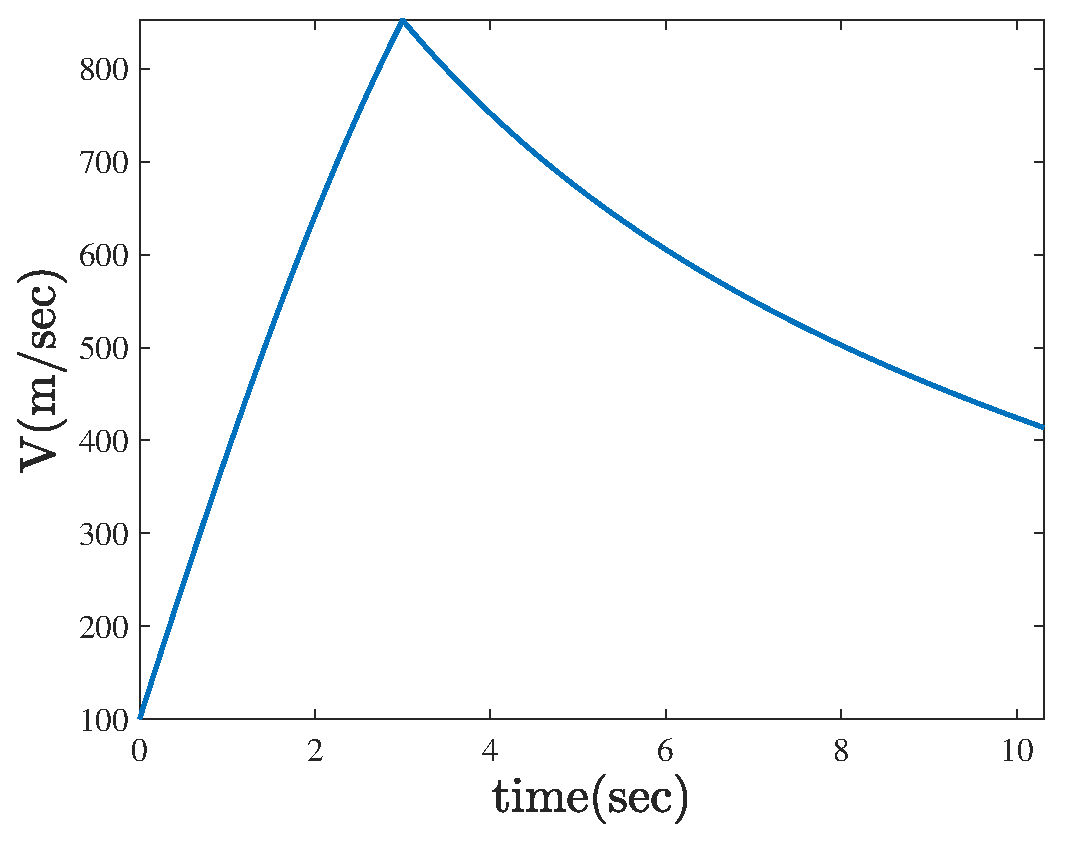
\includegraphics[width=.75\linewidth]{../Figure/d/missle_V}
	\caption{سرعت موشک  در هدایت خط دید پایه همراه با مشتق‌گیر}
\end{figure}

\begin{figure}[H]
	\centering
	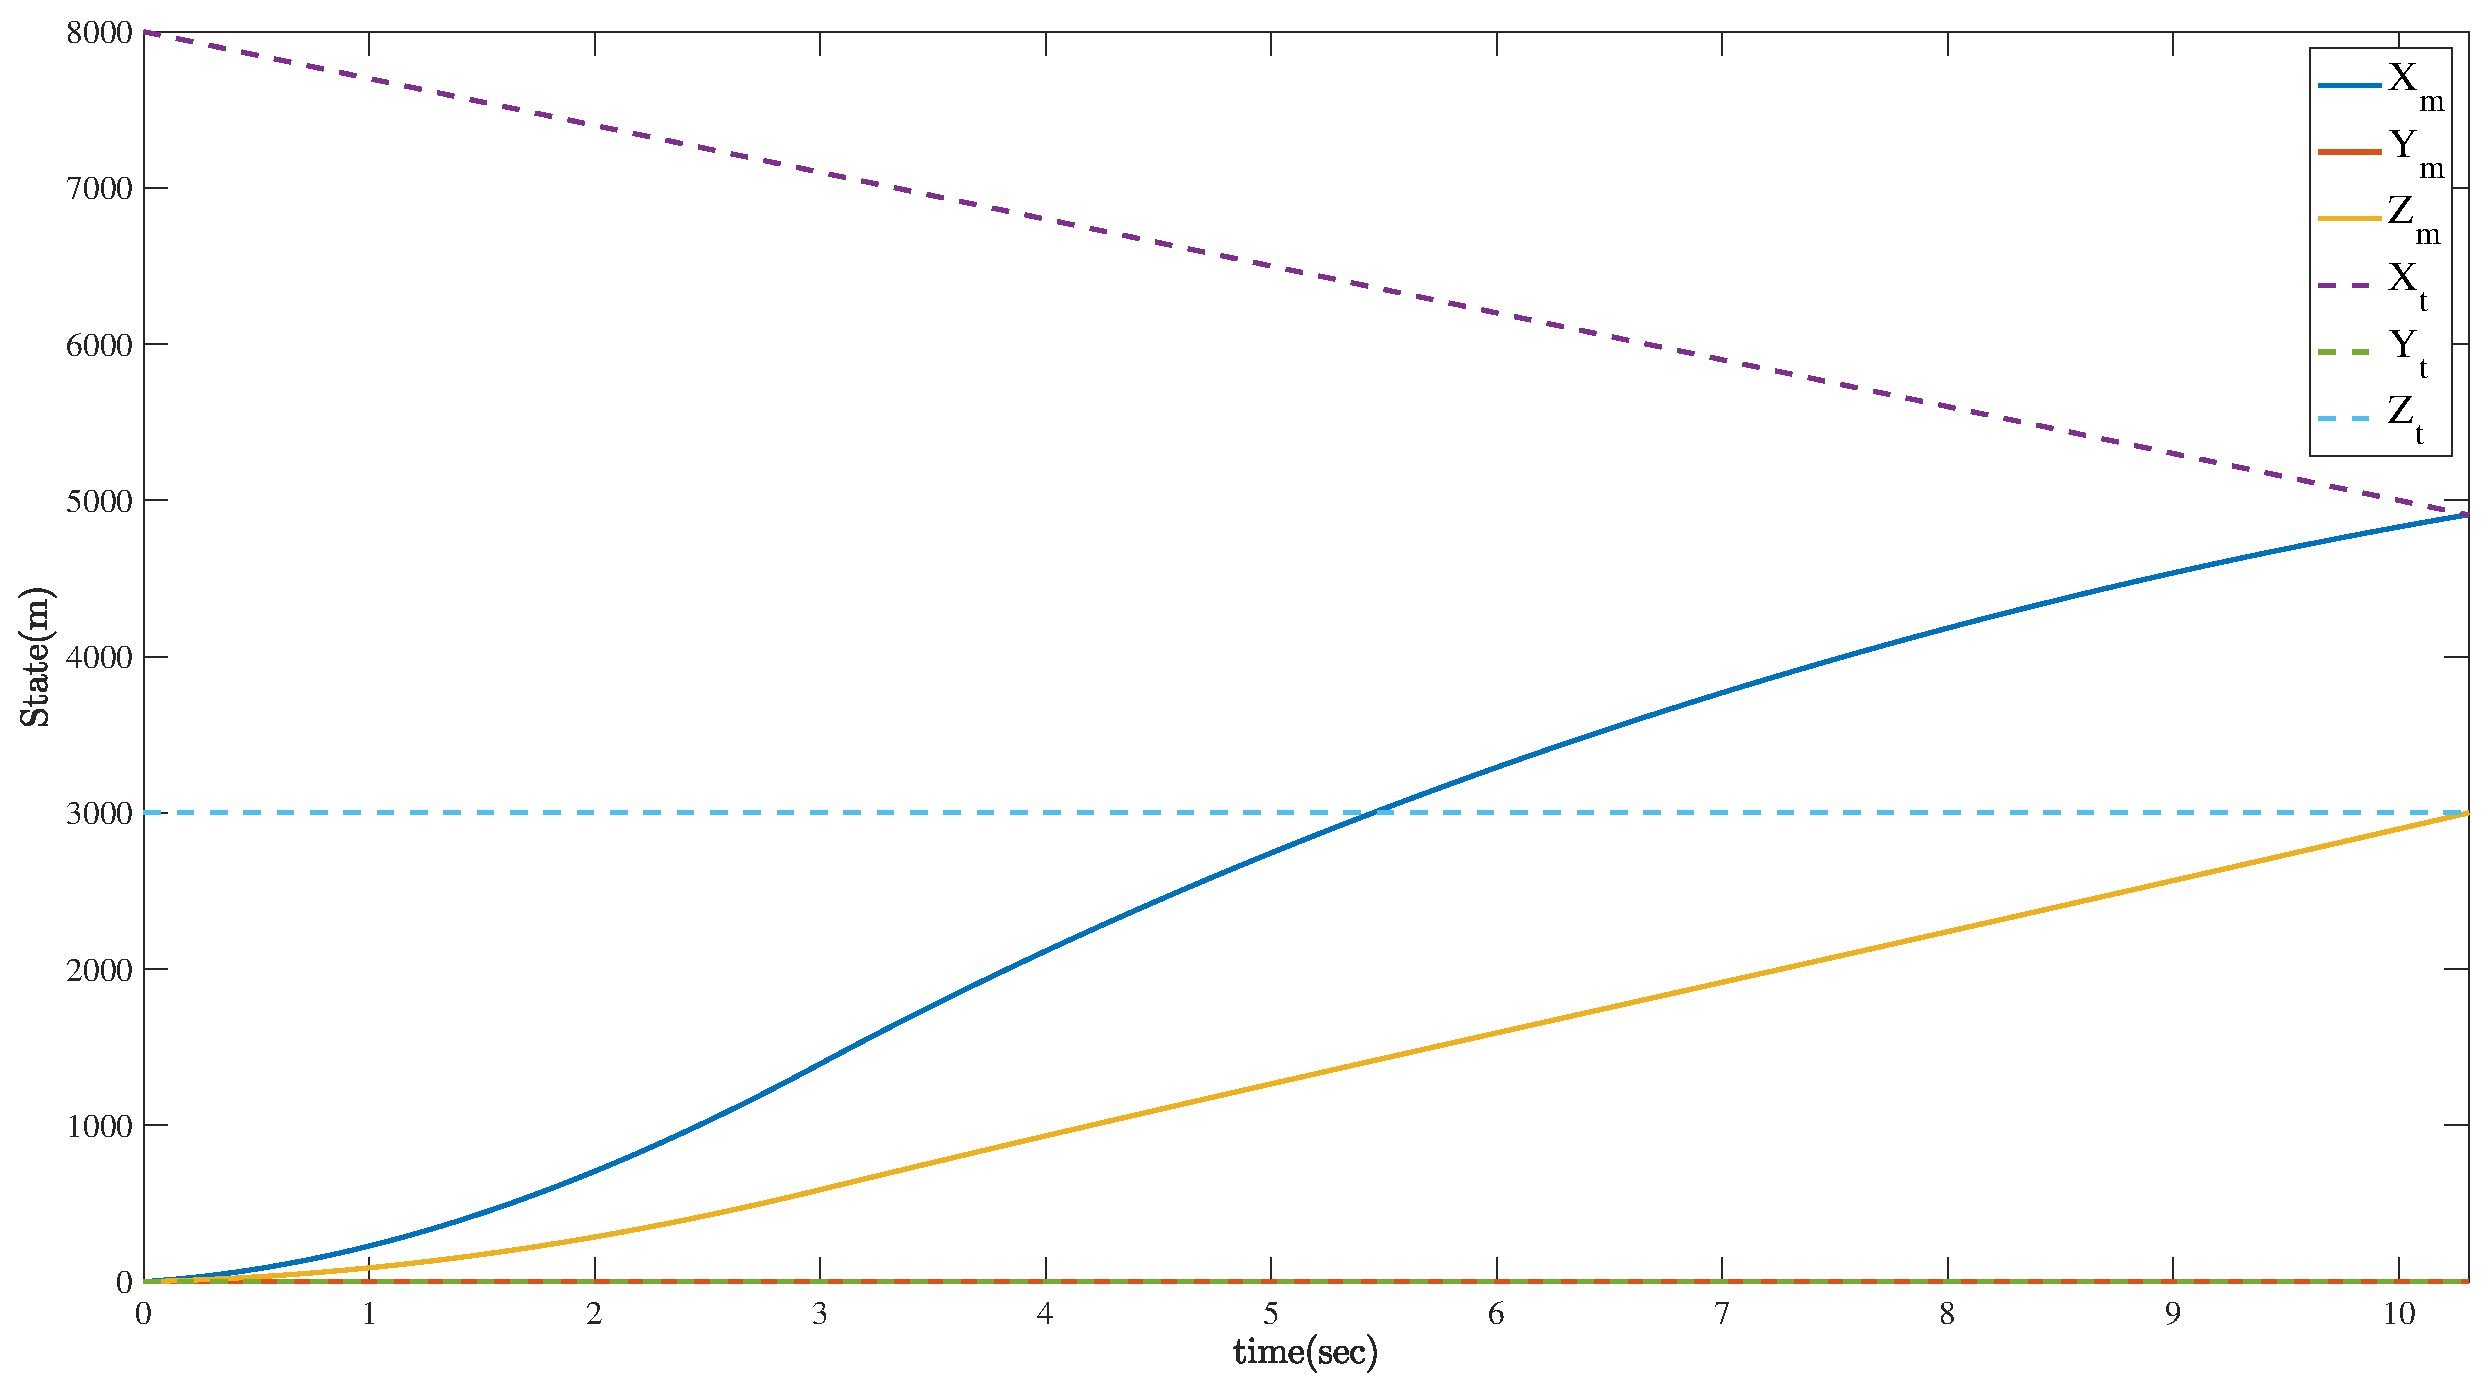
\includegraphics[width=\linewidth]{../Figure/d/missle_vs_target_state}
	\caption{موقعیت موشک و هدف  در هدایت خط دید پایه همراه با مشتق‌گیر}
\end{figure}

\begin{figure}[H]
	\centering
	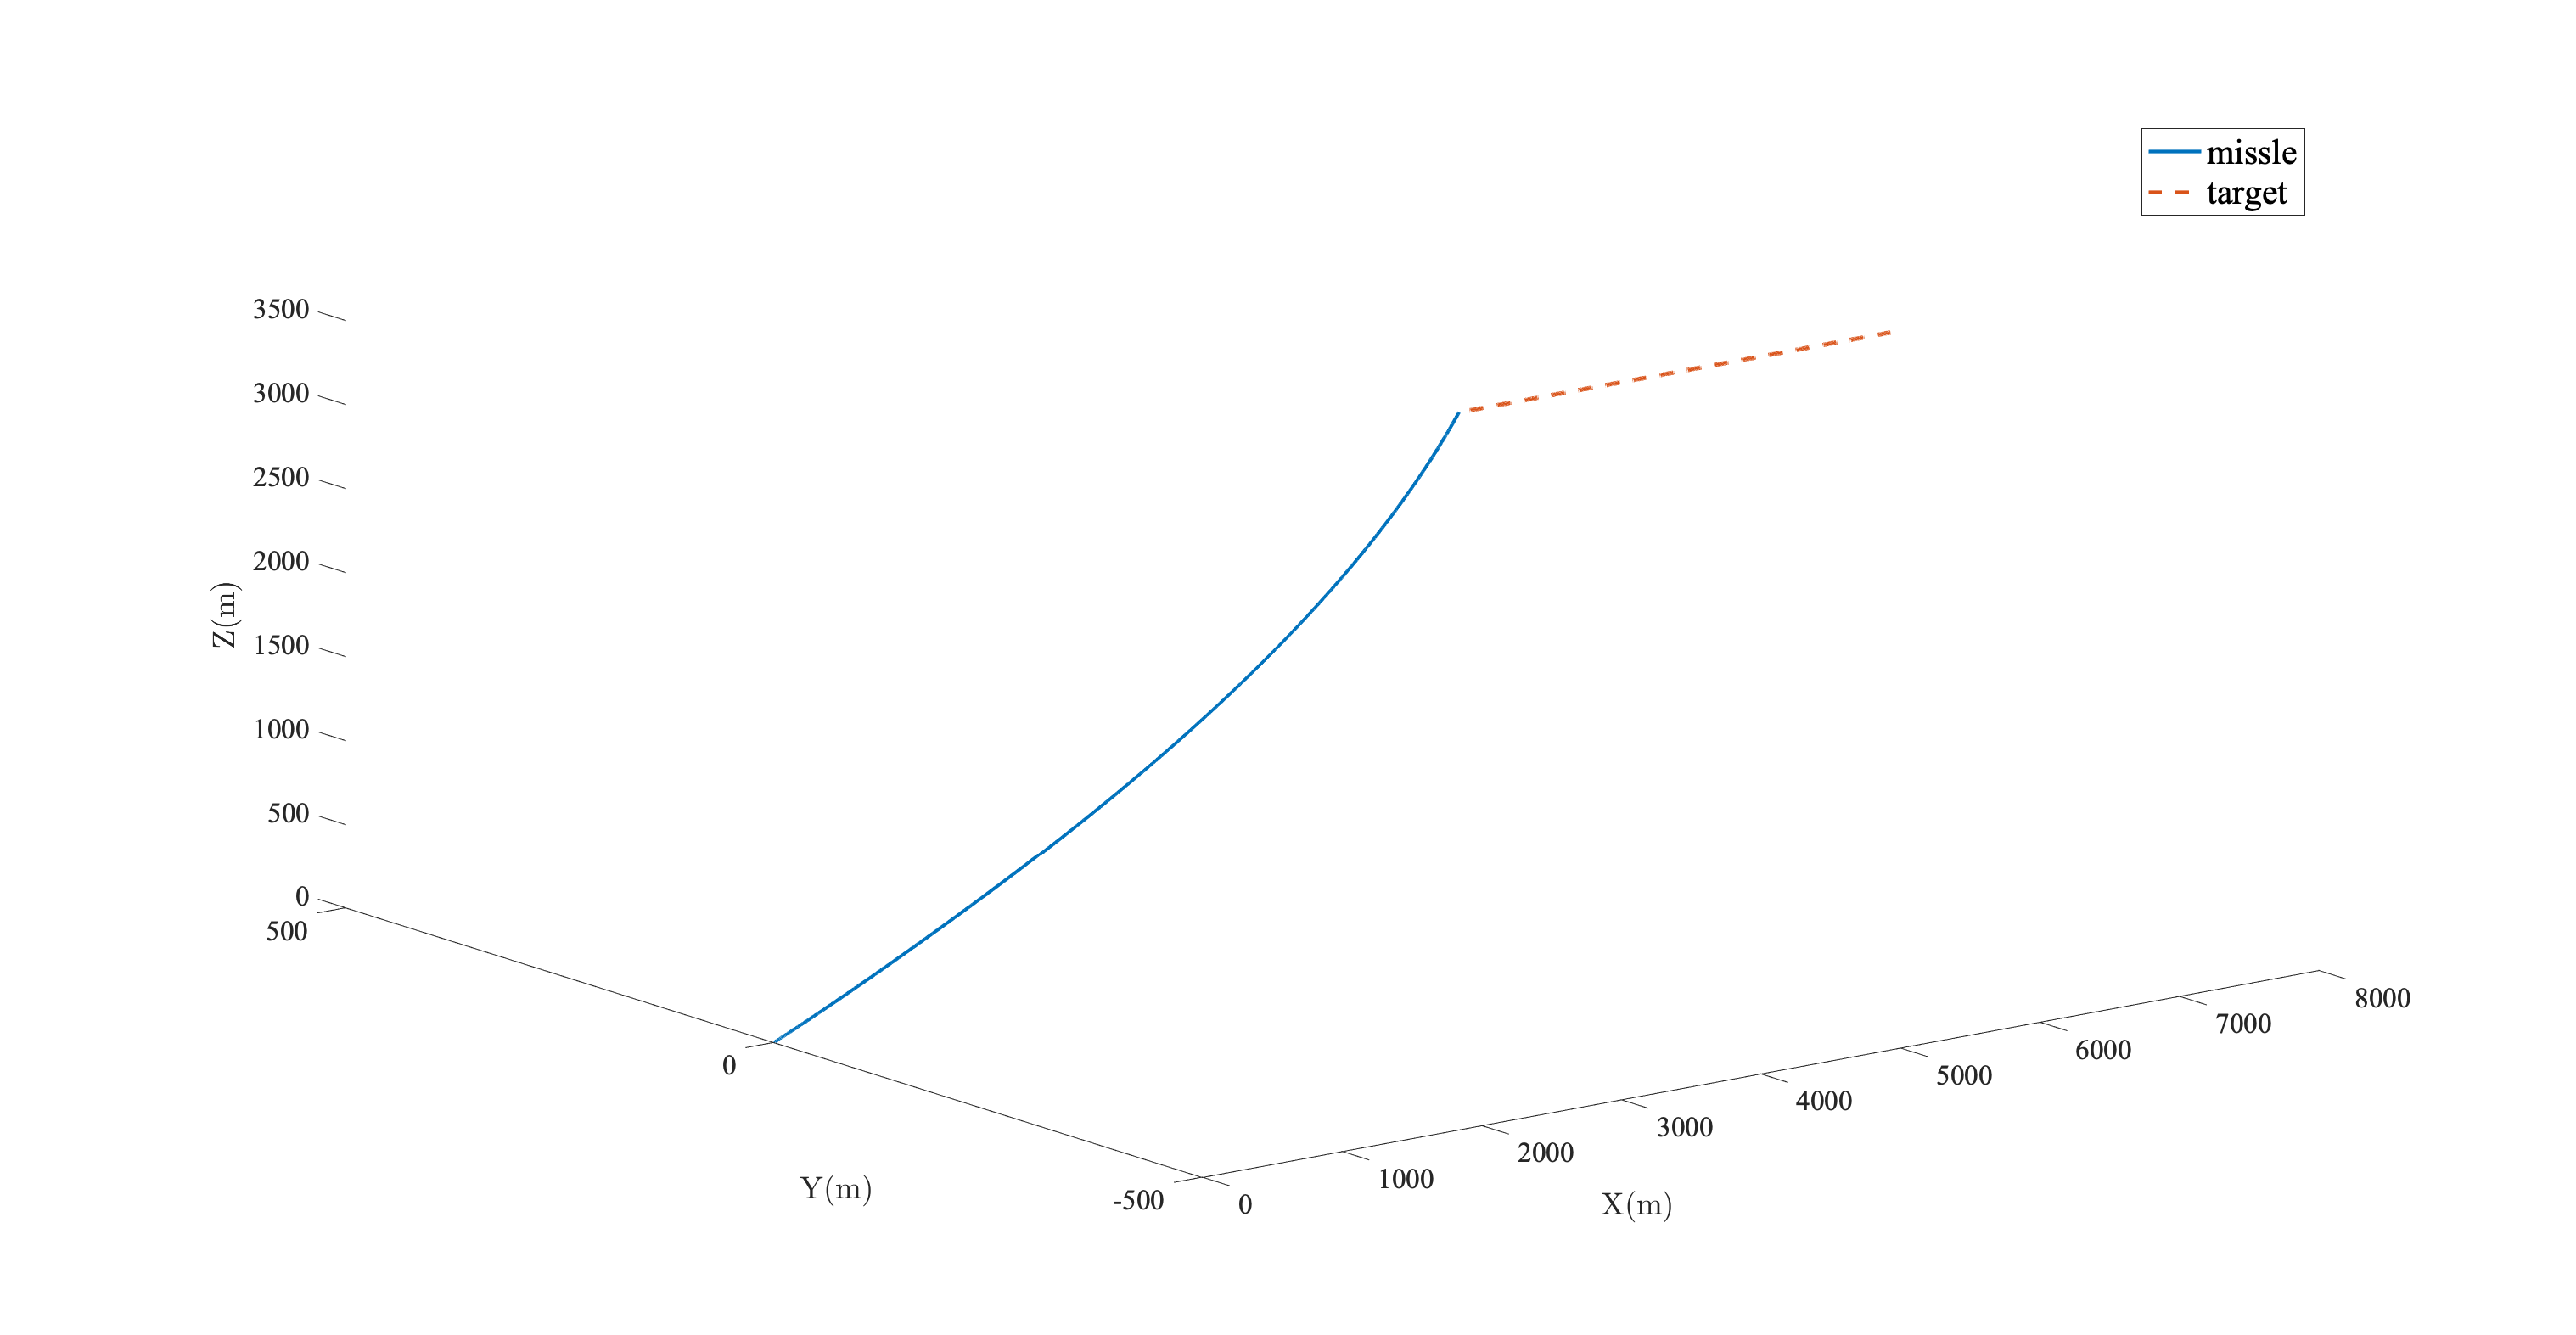
\includegraphics[width=\linewidth]{../Figure/d/3DoF_missle_vs_target_state}
	\caption{موقعیت موشک و هدف به صورت سه بعدی  در هدایت خط دید پایه همراه با مشتق‌گیر}
\end{figure}

\begin{figure}[H]
	\centering
	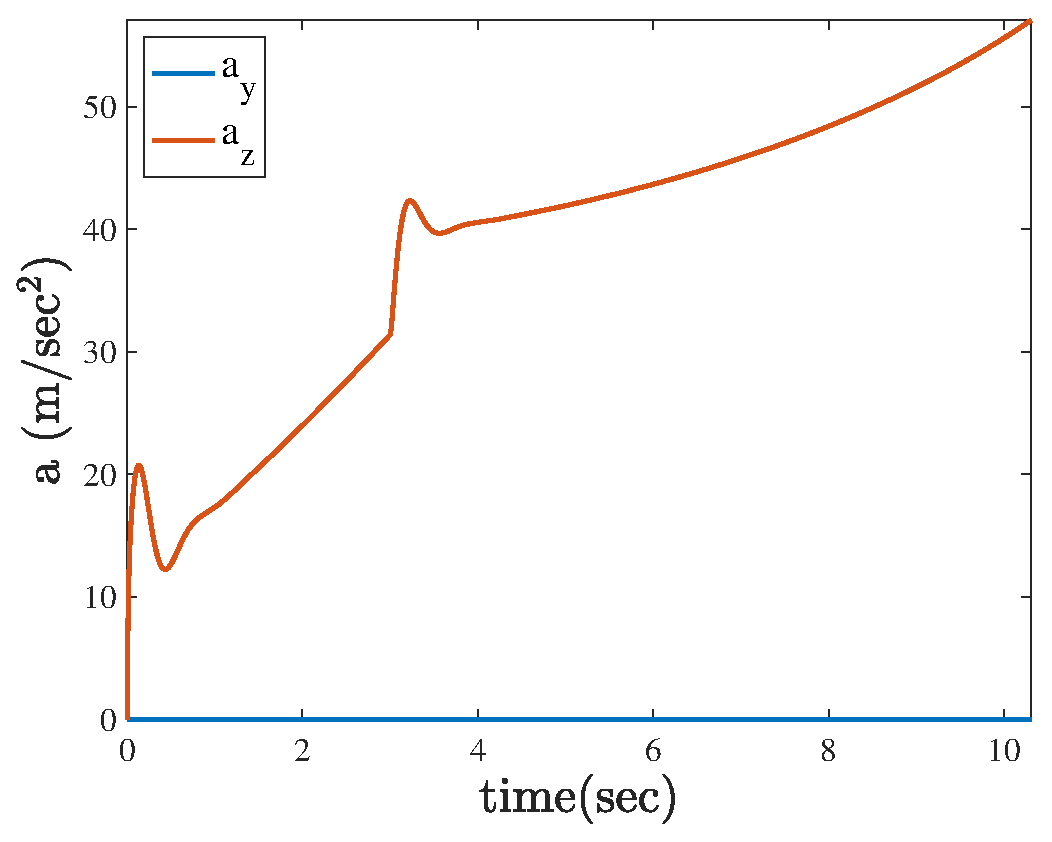
\includegraphics[width=.75\linewidth]{../Figure/d/command}
	\caption{فرمان شتاب در هدایت خط دید پایه همراه با مشتق‌گیر}
\end{figure}

\begin{figure}[H]
	\centering
	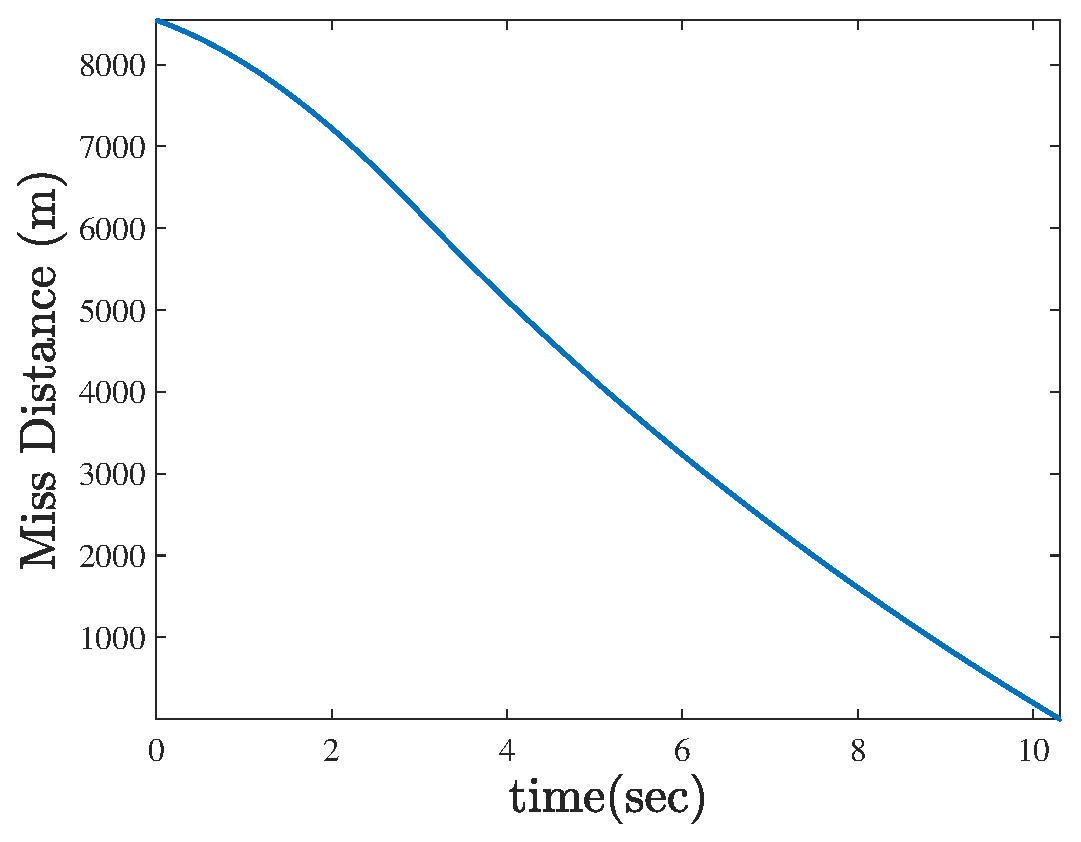
\includegraphics[width=.75\linewidth]{../Figure/d/miss_distance}
	\caption{فاصله ازدست‌دهی در هدایت خط دید پایه همراه با مشتق‌گیر}
\end{figure}


